% Options for packages loaded elsewhere
\PassOptionsToPackage{unicode}{hyperref}
\PassOptionsToPackage{hyphens}{url}
\PassOptionsToPackage{dvipsnames,svgnames,x11names}{xcolor}
\documentclass[
  11pt,
]{article}
\usepackage{xcolor}
\usepackage[margin=1in]{geometry}
\usepackage{amsmath,amssymb}
\setcounter{secnumdepth}{-\maxdimen} % remove section numbering
\usepackage{iftex}
\ifPDFTeX
  \usepackage[T1]{fontenc}
  \usepackage[utf8]{inputenc}
  \usepackage{textcomp} % provide euro and other symbols
\else % if luatex or xetex
  \usepackage{unicode-math} % this also loads fontspec
  \defaultfontfeatures{Scale=MatchLowercase}
  \defaultfontfeatures[\rmfamily]{Ligatures=TeX,Scale=1}
\fi
\ifPDFTeX\usepackage{lmodern}\usepackage{tgtermes}\usepackage{tgheros}\fi
\ifPDFTeX\else
  % xetex/luatex font selection
  \setmainfont[Extension=.otf,UprightFont=*-regular,BoldFont=*-bold,ItalicFont=*-italic,BoldItalicFont=*-bolditalic]{texgyretermes}
  \setsansfont[Extension=.otf,UprightFont=*-regular,BoldFont=*-bold,ItalicFont=*-italic,BoldItalicFont=*-bolditalic]{texgyreheros}
  \setmathfont[]{latinmodern-math.otf}
\fi
% Use upquote if available, for straight quotes in verbatim environments
\IfFileExists{upquote.sty}{\usepackage{upquote}}{}
\IfFileExists{microtype.sty}{% use microtype if available
  \usepackage[]{microtype}
  \UseMicrotypeSet[protrusion]{basicmath} % disable protrusion for tt fonts
}{}
\usepackage{graphicx}
\makeatletter
\newsavebox\pandoc@box
\newcommand*\pandocbounded[1]{% scales image to fit in text height/width
  \sbox\pandoc@box{#1}%
  \Gscale@div\@tempa{\textheight}{\dimexpr\ht\pandoc@box+\dp\pandoc@box\relax}%
  \Gscale@div\@tempb{\linewidth}{\wd\pandoc@box}%
  \ifdim\@tempb\p@<\@tempa\p@\let\@tempa\@tempb\fi% select the smaller of both
  \ifdim\@tempa\p@<\p@\scalebox{\@tempa}{\usebox\pandoc@box}%
  \else\usebox{\pandoc@box}%
  \fi%
}
% Set default figure placement to htbp
\def\fps@figure{htbp}
\makeatother
\setlength{\emergencystretch}{3em} % prevent overfull lines
\providecommand{\tightlist}{%
  \setlength{\itemsep}{0pt}\setlength{\parskip}{0pt}}
% Paper-style layout for the report: Times text, Helvetica figure text, three-line tables, numbered captions.
\usepackage{booktabs,tabularx,array,ragged2e,float,longtable}
\usepackage[font=small,labelfont=bf,labelsep=period,skip=5pt]{caption}
\captionsetup[table]{position=top}
\usepackage{titlesec}
\titleformat{\section}{\normalfont\large\bfseries}{}{0pt}{}
\titleformat{\subsection}{\normalfont\normalsize\bfseries}{}{0pt}{}
\titleformat{\subsubsection}{\normalfont\normalsize\bfseries\itshape}{}{0pt}{}
\titlespacing*{\section}{0pt}{14pt plus 4pt minus 2pt}{6pt plus 2pt}
\titlespacing*{\subsection}{0pt}{10pt plus 3pt minus 2pt}{4pt plus 2pt}
\makeatletter\def\fps@figure{!htbp}\def\fps@table{!htbp}\makeatother
\renewcommand{\topfraction}{0.9}\renewcommand{\bottomfraction}{0.8}
\renewcommand{\textfraction}{0.1}\renewcommand{\floatpagefraction}{0.8}
\setlength{\textfloatsep}{12pt plus 2pt minus 4pt}
\setlength{\floatsep}{10pt plus 2pt minus 2pt}
\renewcommand{\arraystretch}{1.15}
\usepackage{enumitem}
\setlist{itemsep=2pt,topsep=4pt,parsep=0pt}
\usepackage{newunicodechar}
\newunicodechar{−}{\ensuremath{-}}
\newunicodechar{→}{\ensuremath{\rightarrow}}
\newunicodechar{≥}{\ensuremath{\geq}}
\newunicodechar{≈}{\ensuremath{\approx}}
\usepackage{xurl}
\usepackage{titling}
\setlength{\droptitle}{-3em}
\pretitle{\begin{center}\LARGE\bfseries}\posttitle{\par\end{center}\vspace{-0.6em}}
\preauthor{\begin{center}\normalsize}\postauthor{\par\end{center}\vspace{-1.2em}}
\predate{\begin{center}\normalsize}\postdate{\par\end{center}\vspace{-0.5em}}
% pdfLaTeX (Overleaf default): characters inputenc does not know
\ifPDFTeX
  \newunicodechar{κ}{\ensuremath{\kappa}}
  \newunicodechar{≤}{\ensuremath{\leq}}
\fi
\usepackage{bookmark}
\IfFileExists{xurl.sty}{\usepackage{xurl}}{} % add URL line breaks if available
\urlstyle{same}
% fallback for those not using the hyperref driver hyperxmp:
\makeatletter
\@ifundefined{xmpquote}{\newcommand{\xmpquote}[1]{#1}}{}
\makeatother
\hypersetup{
  pdftitle={Social media and search signals flag supply events in U.S. fresh produce markets},
  pdfauthor={Jiuyi Zheng, Gan Xu, Zhiguang Liu, Yizhen Wang},
  colorlinks=true,
  linkcolor={black},
  filecolor={Maroon},
  citecolor={Blue},
  urlcolor={[rgb]{0.1,0.25,0.5}},
  pdfcreator={LaTeX via pandoc}}

\title{Social media and search signals flag supply events in U.S. fresh produce markets}
\usepackage{etoolbox}
\makeatletter
\providecommand{\subtitle}[1]{% add subtitle to \maketitle
  \apptocmd{\@title}{\par {\large #1 \par}}{}{}
}
\makeatother
\subtitle{Cultivate IQ -- NAFSI Track 3 (Supply Chain)}
\author{Jiuyi Zheng, Gan Xu, Zhiguang Liu, Yizhen Wang}
\date{November 2026}

\begin{document}
\maketitle
\begin{abstract}
Reddit talk and Google searches about a product's supply spike when
something happens to that supply. Neither improved price forecasts in our tests. Reddit posts
and comments on
avocados, lettuce, onions and cucumbers from 2019 to 2026 were classified
as price, supply or demand talk, and the weekly amounts were compared
with USDA wholesale prices and shipments around 33 documented market
events.
Spikes in Reddit supply talk fell near these events twice as often as
chance, and US Google searches for shortages and recalls spiked in the
same weeks. Reddit tells what happened, such as an import halt, a crop disease
or a recall; prices and shipments tell whether it mattered. Every unusual
price rise came with a supply disruption: a border closure threat, a heat
wave, a crop virus, a tariff. No food-safety outbreak, COVID-19 closure
or viral recipe raised prices on its own. Adding Reddit, Google
searches, news coverage, FDA recalls or Wikipedia pageviews to price
history did not improve forecasts of national prices one or four weeks
ahead, and around the events prices often moved before the talk did.
\end{abstract}

\section{1. Introduction}\label{introduction}

Shoppers, grocery staff, cooks and growers write online about
shortages, recalls and price jumps as they meet them. Online text has
tracked such events before: search queries followed influenza (Ginsberg
et al., 2009), and tweets followed food prices in Indonesia (Kim et al.,
2017). In this report, Reddit talk about fresh produce is compared with
USDA Market News wholesale prices and shipments.

Two questions are addressed: whether Reddit shows what lies behind a
U.S. produce price move, and whether it forecasts prices. Avocados,
lettuce (iceberg and romaine), dry onions and cucumbers are studied from
January 2019 to September 2026. All four are perishable, priced every
trading day in every terminal market and often named in conversation.
The eight years cover the COVID-19 closures and enough documented events
to compare event weeks with ordinary weeks and to test forecasts on data
not used for training.
The signal is tested on 33 documented market events chosen by fixed
rules (Table 1, Appendix D).

\begin{table}[htbp]
\centering\small
\caption{Documented events, January 2019 to September 2026, by kind. Each event has a product, dates and a news or agency source (Appendix D).}
\begin{tabularx}{\linewidth}{>{\RaggedRight\arraybackslash\hsize=0.62\hsize}X>{\RaggedRight\arraybackslash\hsize=1.0\hsize}X>{\RaggedRight\arraybackslash\hsize=1.38\hsize}X>{\centering\arraybackslash}p{1.1cm}}
\toprule
Kind & Rule & Examples & Events \\
\midrule
Food-safety outbreaks & Every CDC multistate outbreak linked to one of the products & Salinas romaine E. coli (2019), red onion Salmonella (2020), McDonald's onion E. coli (2024), iceberg Cyclospora (2026) & 10 \\
Supply disruptions & Reported in the produce trade press: import halts, border actions, tariffs, crop disease, weather & US halt of Mexican avocado imports (2022), INSV lettuce virus (2022), tariff on Mexican imports (2025), Florida freeze (2026) & 18 \\
Demand shocks & Reported nationally & COVID-19 closures (2020, one event per product), viral cucumber salad (2024) & 5 \\
\bottomrule
\end{tabularx}
\end{table}

Figure 1 shows two cases from 2022. When the United States
halted Mexican avocado imports, Reddit carried the news the next day;
shipments then fell and prices rose. When a virus cut California lettuce
yields, a restaurant worker described the disease in August, but most
talk came in November, when prices peaked. In both cases Reddit told what
happened, and prices and shipments told how much it mattered. Sections
3.1--3.2 test this pattern on all 33 events, and Sections 3.3--3.4 test
whether online talk forecasts prices.

\begin{figure}
\centering
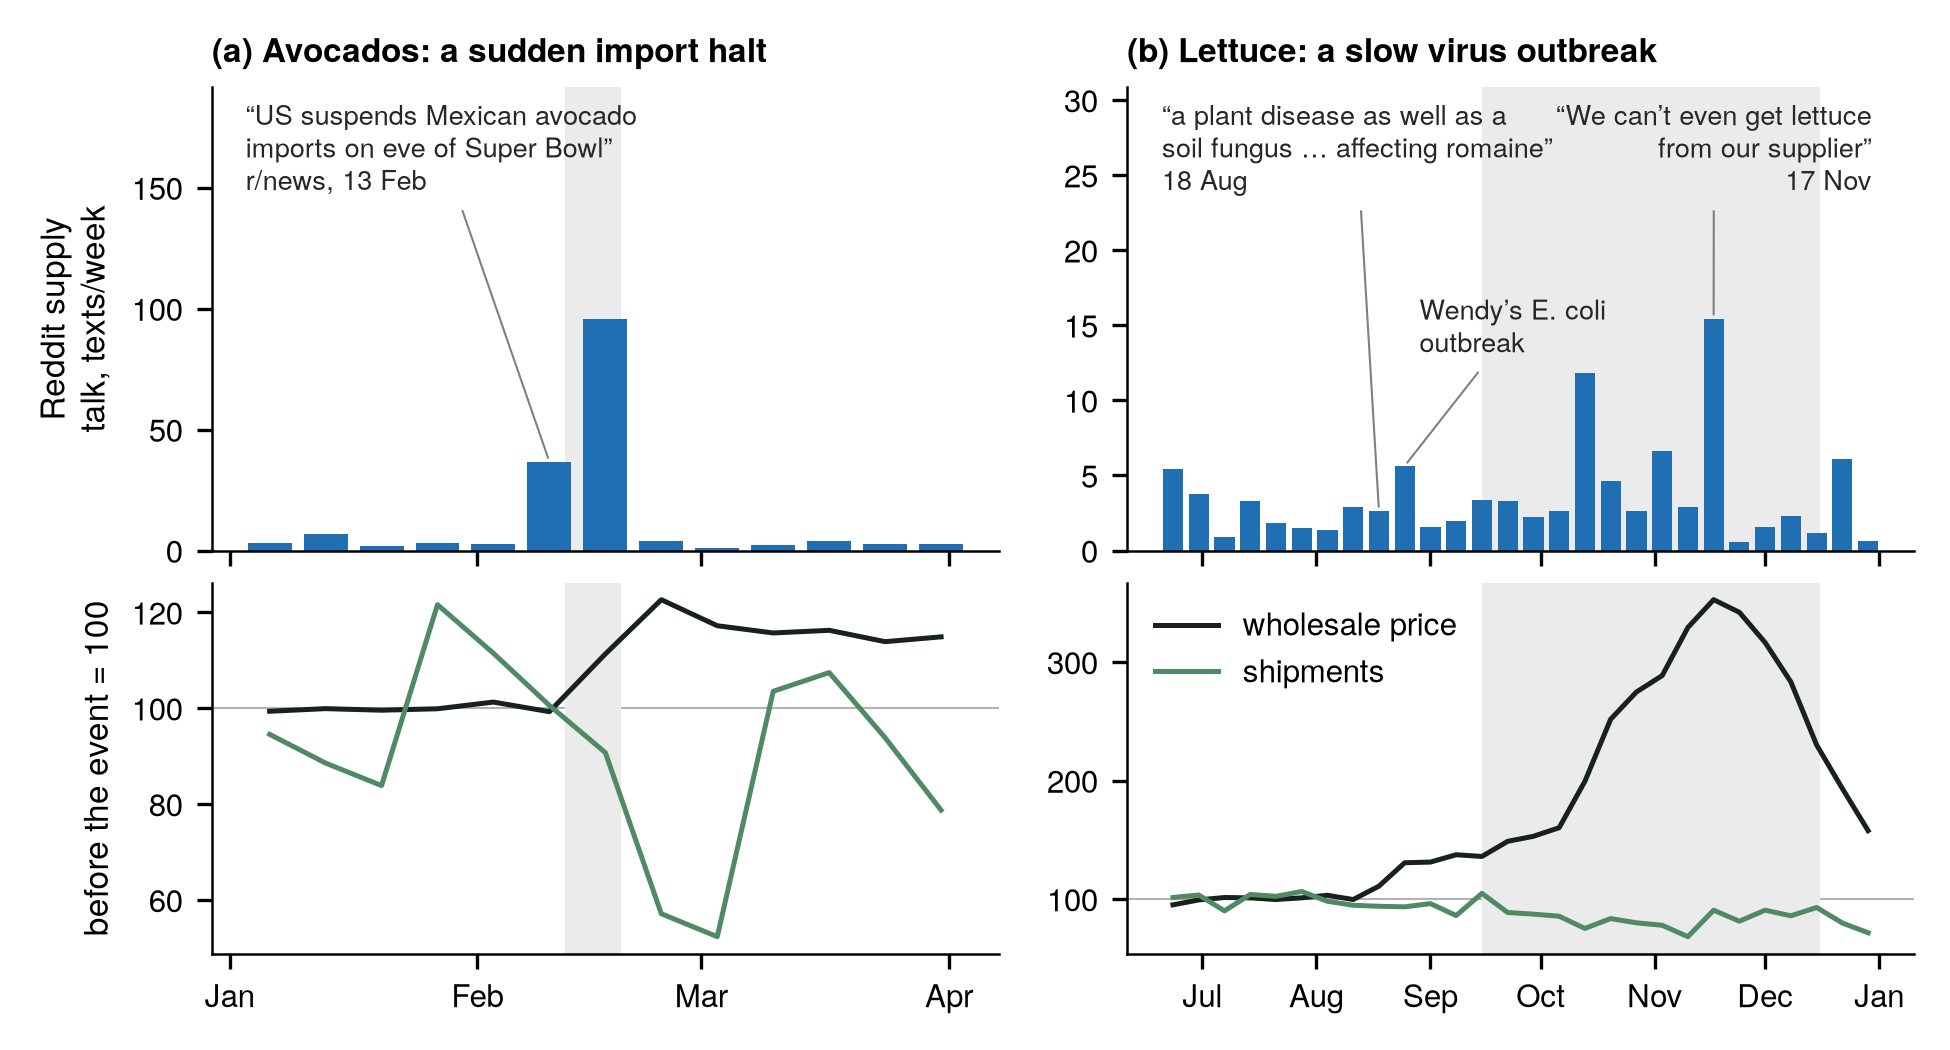
\includegraphics[width=1\linewidth,height=\textheight,keepaspectratio,alt={Two
supply shocks up close. Top: weekly Reddit supply talk, with quotes from
Reddit posts. Bottom: national wholesale price and shipments, each
scaled to 100 before the event. Grey bands mark the
events.}]{../outputs/figures/two_supply_shocks.png}
\caption{Two supply shocks up close. Top: weekly Reddit supply talk,
with quotes from Reddit posts. Bottom: national wholesale price and
shipments, each scaled to 100 before the event. Grey bands mark the
events.}
\end{figure}

\section{2. Data and methods}\label{data-and-methods}

\begin{figure}
\centering
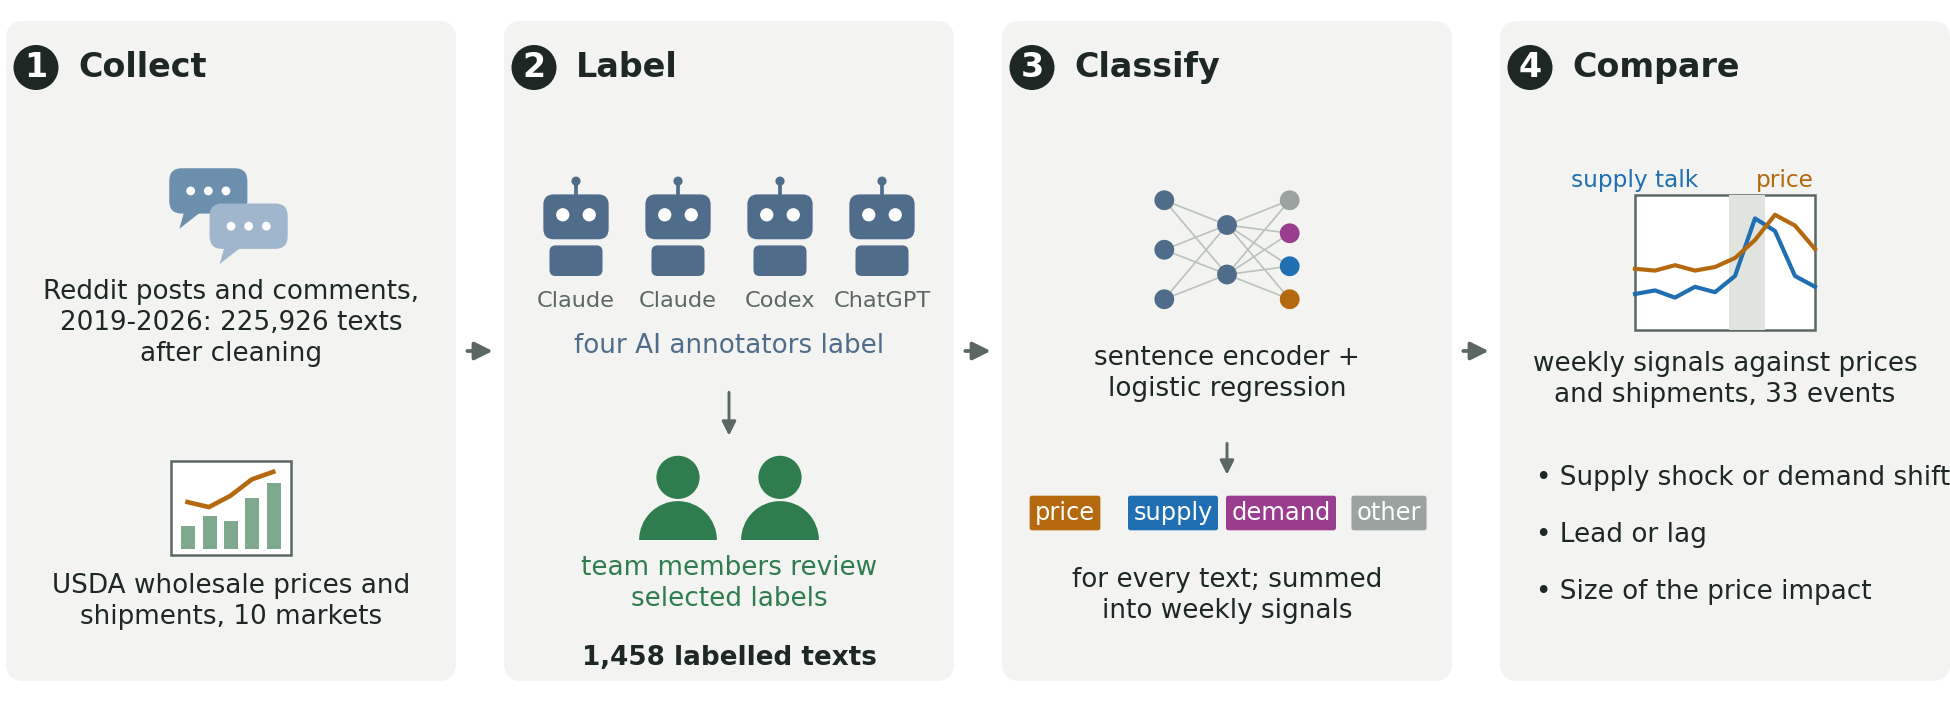
\includegraphics[width=1\linewidth,height=\textheight,keepaspectratio,alt={Study
workflow. Four AI annotators label a sample of texts, and team members
review selected cases. A classifier trained on these labels
classifies every text, and its weekly signals are compared with USDA
prices and shipments around documented
events.}]{../outputs/figures/data_workflow.png}
\caption{Study workflow. Four AI annotators label a sample of texts, and
team members review selected labels. A classifier trained on these
labels classifies every text, and its weekly signals are compared with
USDA prices and shipments around documented events.}
\end{figure}

\textbf{Data.} Reddit posts are public and timestamped. Posts from
topical and city subreddits, the comments under product threads, and
r/news headlines were collected through the Arctic Shift archive (Table
2). Bots, moderator notices, crossposts, paid and self-promotion, link
farms, very short texts and duplicates were removed (Appendix A). The remaining texts form the
event dataset. Each row is one text and one product it names, with the
date, subreddit, city where known, and the event types its words match
in the keyword dictionary (price change, supply shortage, demand change,
weather, food-safety recall, promotion). A summary table counts the rows
by product and event type (Appendix F). USDA AMS gives the market side:
daily wholesale prices, combined into a weekly price index per product, and weekly shipments from US growing regions and imports.
Prices and shipments together tell a supply shock from a demand shift.
Google Trends gives a second online signal: weekly US searches for each
product alone and with ``price'', ``shortage'' and ``recall''. Every
source was collected from January 2019 to September 2026 in three
periods with the same pipeline. The forecasting test adds three more free
sources: US news coverage (GDELT), FDA food recalls (openFDA) and
Wikipedia pageviews.

\begin{table}[htbp]
\centering\small
\caption{Data sources, January 2019 to September 2026.}
\begin{tabularx}{\linewidth}{>{\RaggedRight\arraybackslash\hsize=0.8\hsize}X>{\RaggedRight\arraybackslash\hsize=0.95\hsize}X>{\RaggedRight\arraybackslash\hsize=1.25\hsize}X}
\toprule
Source & Data used & Coverage \\
\midrule
Reddit, via the Arctic Shift archive & Posts, comments and r/news headlines that name a product & 29 topical subreddits (cooking, grocery, food service, growing, economy) and 9 city subreddits; 225,926 texts after cleaning \\
USDA AMS terminal market reports & Daily wholesale prices & 10 cities \\
USDA AMS movement reports & Weekly shipments from US growing regions and imports & National \\
Google Trends & Weekly search interest & US; 4 search terms per product \\
GDELT & Daily news volume and tone & US English-language news; 4 queries per product; forecasting only \\
openFDA & Food recall reports that name a product & US; forecasting only \\
Wikipedia & Daily pageviews of each product's article & English Wikipedia; forecasting only \\
Labelled sample & Texts labelled price, supply, demand or other & 1,458 texts from 2022--2024 \\
\bottomrule
\end{tabularx}
\end{table}

\textbf{Labels.} Each text gets one label for each product it names:
price, supply, demand or other (Appendix B). Supply covers availability,
shortages, crop problems, imports and recalls; avoiding a product after
a scare counts as demand. One text per thread from 2022--2024 was
labelled, most of them drawn with market keywords so that the rare
labels are well represented. Two Claude models labelled the sample; 1,118 texts were also labelled
independently by OpenAI Codex and ChatGPT. The 1,458 reference labels
combine AI agreement with targeted team review: 388 have documented human
review or adjudication, while the remaining 1,070 have AI-agreement or
ChatGPT-confirmed labels (Appendix B). In 100 adjudications, team members
chose between two labels without knowing which model proposed which
(Figure 2).

\textbf{Classifier.} Each text, preceded by the product name, is encoded
with a pretrained sentence encoder (all-mpnet-base-v2) and labelled by a
logistic regression trained on the labelled sample. It beats keyword rules and
the zero-shot model of the challenge example, and matches a fine-tuned
DistilRoBERTa that takes far longer to train (Table 3). The
same model labels the texts of every year. Each
week\textquotesingle s amount of price, supply and demand talk is the
sum of the predicted probabilities over that week\textquotesingle s
texts (Appendix C).

\begin{table}[htbp]
\centering\small
\caption{Classifier accuracy in 5-fold cross-validation, grouped by Reddit thread.}
\begin{tabular}{lcc}
\toprule
Model & Macro-F1 & Accuracy \\
\midrule
Zero-shot BART-large-MNLI (challenge example) & 0.34 & 24\% \\
Keyword rules (Task 1 dictionary) & 0.39 & 40\% \\
Fine-tuned DistilRoBERTa & 0.71 & 75\% \\
\textbf{all-mpnet + logistic regression (ours)} & \textbf{0.72} & \textbf{82\%} \\
\bottomrule
\end{tabular}
\end{table}

\section{3. Results}\label{results}

\subsection{3.1 Supply talk spikes near real
events}\label{supply-talk-spikes-near-real-events}

Spikes in supply talk point to real events. A week is counted as a spike
when a series rises at least three standard deviations above its previous
eight weeks. Supply-talk spikes fall within two weeks of a documented
event twice as often as chance (Table 4). Spikes in price talk, demand
talk, overall volume or sentiment are no more common near events than
chance would give. Supply talk spiked around 20 of the 33 events, among them 9 of
the 10 food-safety outbreaks, when people passed on recall notices
(Figure 3).

\begin{table}[htbp]
\centering\small
\caption{Spikes of at least three standard deviations above the previous eight weeks, January 2019 to September 2026, and how many lie within two weeks of a documented event. By chance, 21\% of weeks would.}
\begin{tabular}{lccc}
\toprule
Series & Spike weeks & Near an event & p \\
\midrule
Reddit supply talk & 55 & 23 (42\%) & 0.0003 \\
Reddit price talk & 47 & 14 (30\%) & 0.10 \\
Reddit demand talk & 55 & 14 (25\%) & 0.24 \\
Reddit overall volume & 54 & 13 (24\%) & 0.33 \\
Reddit sentiment, either direction & 52 & 13 (25\%) & 0.28 \\
Google searches, shortage or recall & 84 & 35 (42\%) & \textless{} 0.0001 \\
\bottomrule
\end{tabular}
\end{table}

\begin{figure}
\centering
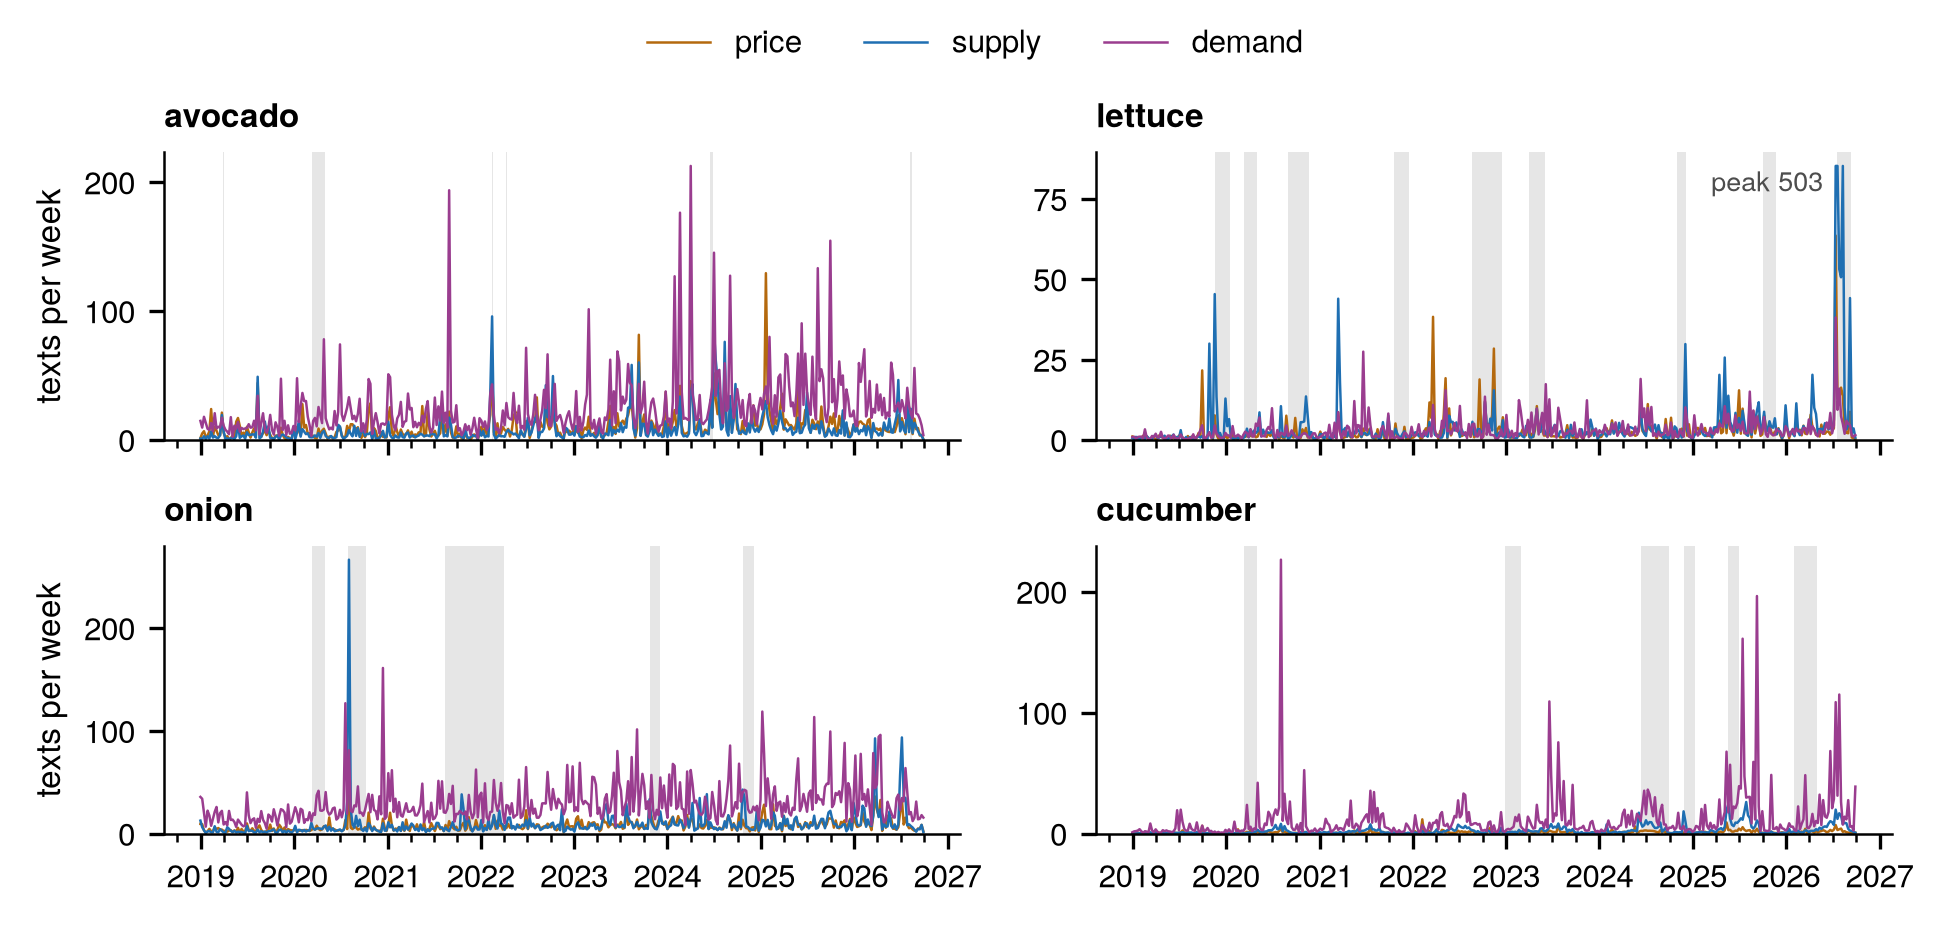
\includegraphics[width=1\linewidth,height=\textheight,keepaspectratio,alt={Weekly
amount of price, supply and demand talk on Reddit per product (summed
classifier probabilities). Grey bands mark the documented
events.}]{../outputs/figures/weekly_signals.png}
\caption{Weekly amount of price, supply and demand talk on Reddit per
product (summed classifier probabilities). Grey bands mark the documented
events. The lettuce axis is cut at the July 2026 Cyclospora outbreak.}
\end{figure}

US Google searches confirm the pattern. Searches for a
product\textquotesingle s shortage or recall spike near documented
events as often as Reddit supply talk does (Table 4, Appendix E). Reddit
or Google spiked around 24 of the 33 events, and in 13 of them the two
peaked in the same week. Counting texts by their upvotes or comments
finds no more events than counting each text once (Appendix G).

\subsection{3.2 Prices show which events
mattered}\label{prices-show-which-events-mattered}

Every unusual price rise came with a supply disruption. A supply shock
raises prices while shipments fall; a demand shift moves prices and
shipments in the same direction. For each event, the event weeks and
the two weeks after were compared with the eight weeks before, net of the
same weeks two years before and after, and the change was ranked among
all other windows of the same length (Table 5, Figure 4). Prices rose more
than in nine of ten ordinary windows in eight events, all during supply
disruptions. In six of them shipments fell as well. A carton of 48 Hass
avocados went from \$30 to \$60 when the border closure was threatened in
2019, and a carton of 24 iceberg heads from \$30 to \$68 during the 2022
lettuce virus. No food-safety outbreak, COVID-19 closure or viral recipe
raised prices on its own; the 2024 SunFed recall and the COVID-19
closures lowered cucumber prices.

\begin{table}[htbp]
\centering\small
\caption{Events with an unusual price change: change in price and shipments over the event and the two weeks after, relative to the eight weeks before and beyond the seasonal norm. Supply talk: whether Reddit supply talk rose during the event.}
\begin{tabularx}{\linewidth}{>{\RaggedRight\arraybackslash}Xcccl}
\toprule
Event & Price & Shipments & Supply talk & Market reading \\
\midrule
E15 Lettuce virus (INSV), 2022 & +121\% & −13\% & rose & \textbf{Supply shock} \\
E14 Wendy's romaine outbreak, 2022, start of E15 & +69\% & −11\% & -- & \textbf{Supply shock} \\
E9 Northwest heat wave, onion crop, 2021--22 & +41\% & −20\% & rose & \textbf{Supply shock} \\
E1 US--Mexico border closure threat, avocado, 2019 & +40\% & −12\% & rose & \textbf{Supply shock} \\
E11 Onion Salmonella outbreak, 2021, inside E9 & +22\% & −9\% & rose & \textbf{Supply shock} \\
E26 Tariff on Mexican imports, cucumber, 2025 & +19\% & −32\% & -- & \textbf{Supply shock} \\
E30 Salinas lettuce shortage, 2025 & +83\% & 0\% & -- & Price rise, shipments level \\
E31 Florida freeze, cucumber, 2026 & +37\% & +1\% & -- & Price rise, shipments level \\
E24 SunFed cucumber recall, 2024 & −25\% & +3\% & rose & Demand fall \\
E4 COVID-19 closures, cucumber, 2020 & −15\% & −8\% & -- & Demand fall \\
\bottomrule
\end{tabularx}
\end{table}

\begin{figure}
\centering
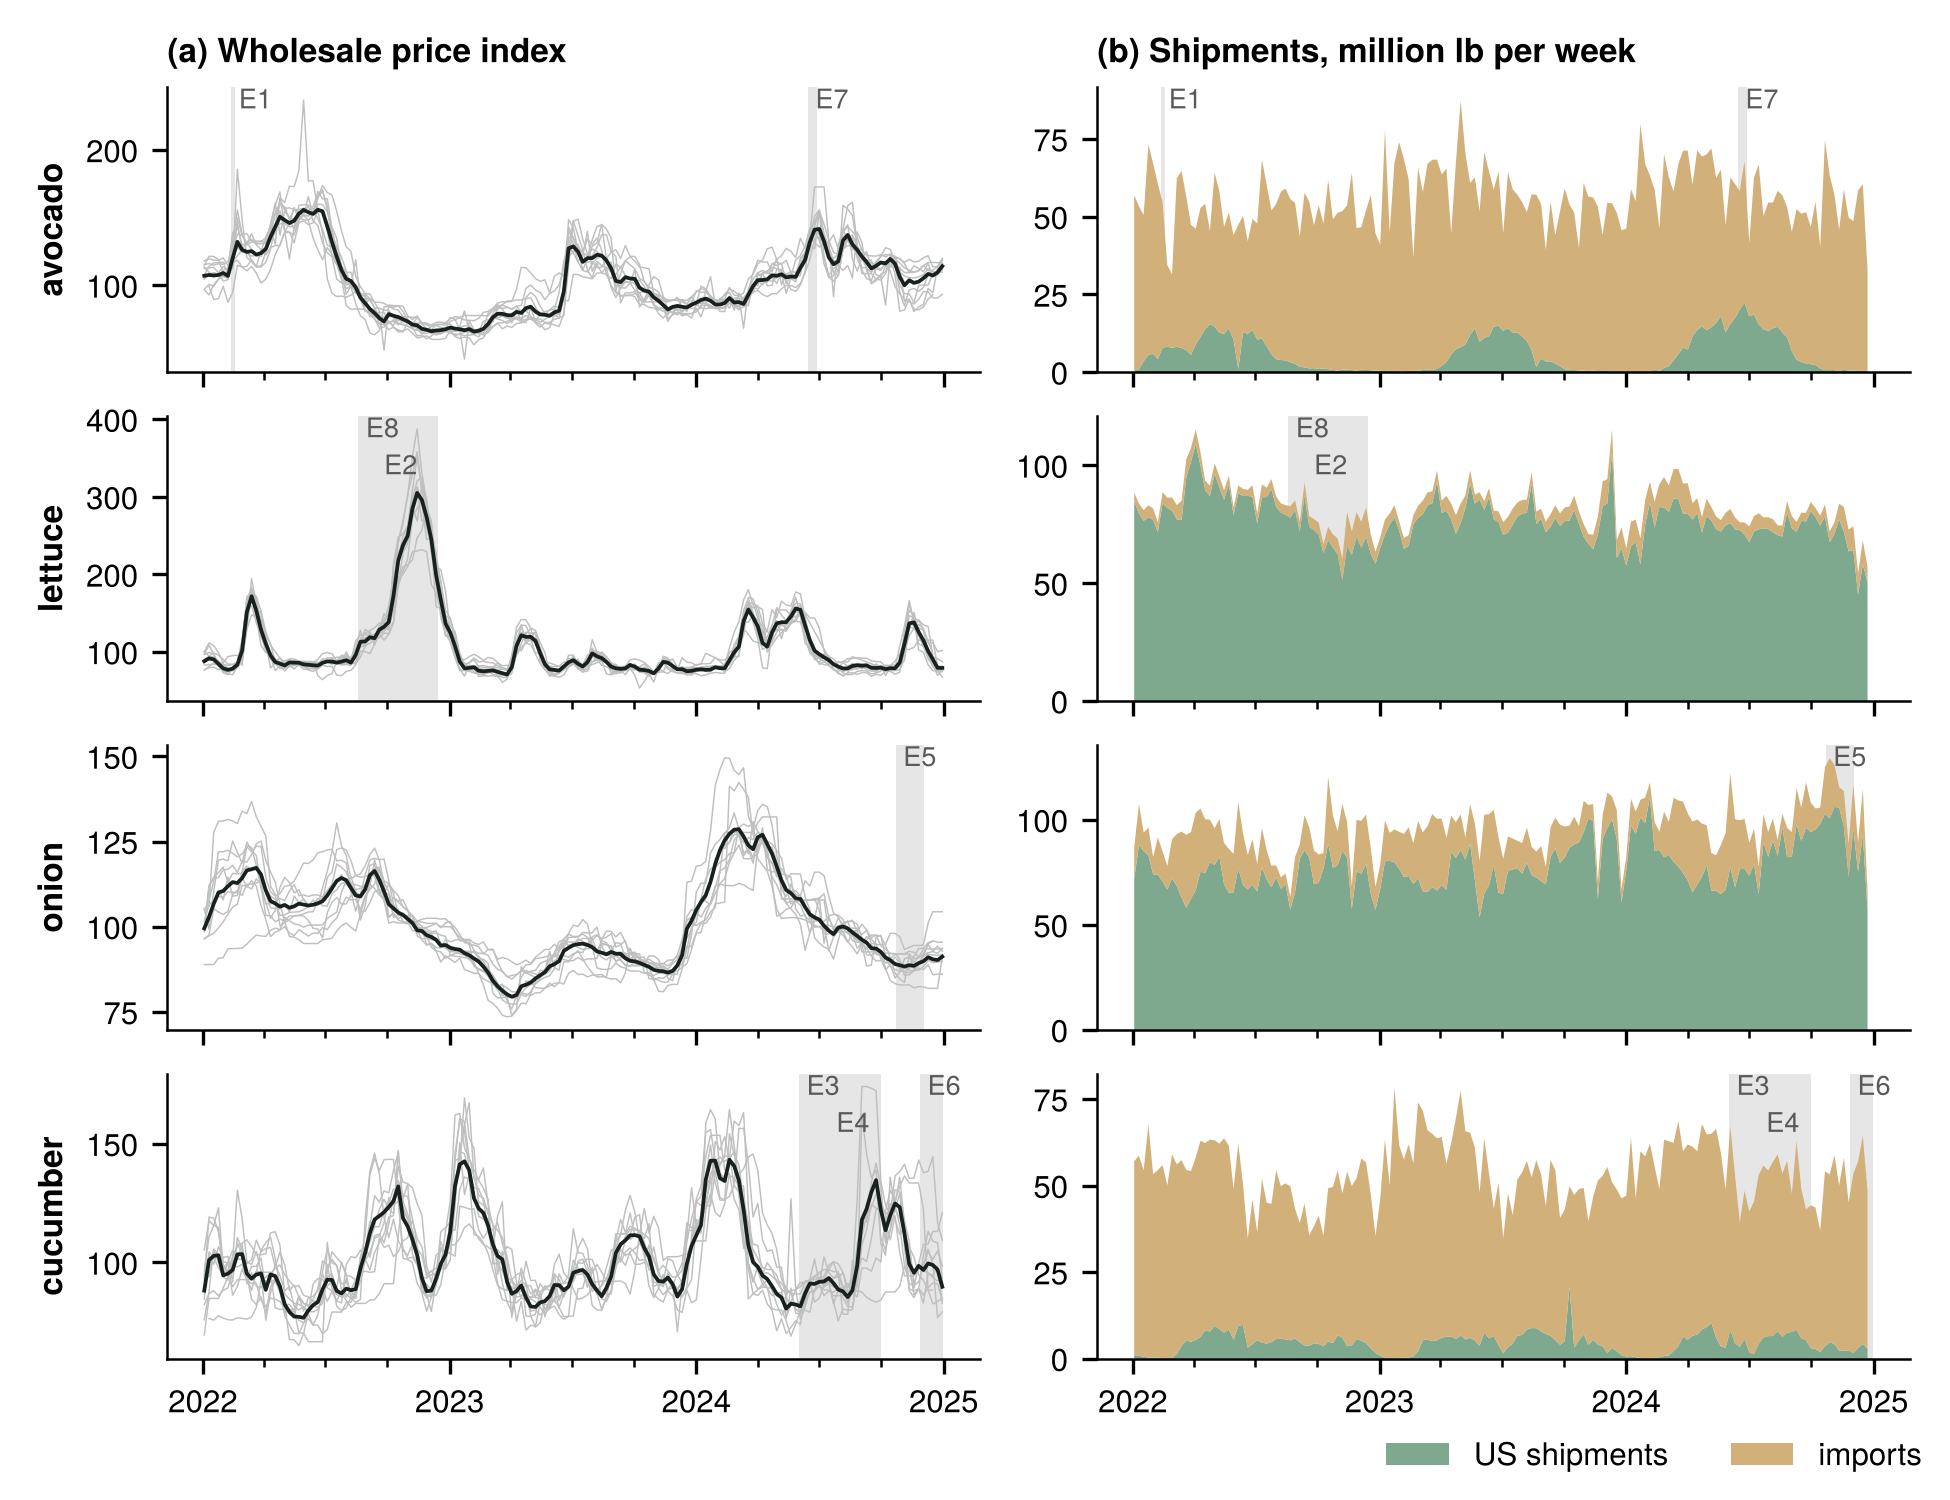
\includegraphics[width=1\linewidth,height=\textheight,keepaspectratio,alt={(a)
Wholesale price index per product: all ten terminal markets pooled
(black) and each market (grey), scaled to a 2019--2026 mean of about
100. (b) Weekly shipments from US growing regions and imports. Grey
bands mark the documented events.}]{../outputs/figures/prices_and_shipments.png}
\caption{(a) Wholesale price index per product: all ten terminal markets
pooled (black) and each market (grey), scaled to a 2019--2026 mean of
about 100. (b) Weekly shipments from US growing regions and imports.
Grey bands mark the documented events.}
\end{figure}

The other 21 events with a measured effect moved national prices no more
than ordinary weeks do. Among them is the 2022 avocado import halt: it cut
shipments by a quarter, and its price rise was within the ordinary range.

\subsection{3.3 Online signals did not improve tested forecasts}\label{online-signals-do-not-forecast-prices}

None of the tested online sources improved national wholesale-price forecasts
beyond price history. For each week from
January 2021 to September 2026, the national price index one and four
weeks ahead, and whether it would make a big move, were forecast with
models trained only on earlier weeks. Each model used price history alone or
price history plus one online source. The best forecasts use price
history alone; no source improves them, and adding all sources together
does not help either (Appendix H). Talk around the documented events
shows the same (Section 3.4).

\subsection{3.4 Talk does not lead prices}\label{talk-does-not-lead-prices}

Reddit reports sudden shocks at once and explains slow ones as they
peak. The avocado import halt was announced on Saturday, 12 February
2022. Supply talk surged the next day, mostly in r/news, and wholesale
prices rose the following week (Figure 1a). The lettuce shortage built
up over months. Prices began to climb in mid-August 2022, the week a
restaurant worker wrote that a plant disease and a soil fungus were
hitting lettuce in the Salinas growing region. The rise in lettuce talk
later that month was about the Wendy\textquotesingle s outbreak (Figure
1b). Most talk about the shortage itself came in mid-November, the week
prices peaked: supplier outages, romaine at \$5 a head, restaurant
chains warning customers. Across all events, talk did not lead prices.
In 27 events both moved. Prices moved more than a week before supply
talk in 12, within a week of it in 8, and after it in 7; the median gap
was one week, with prices first. Across all
weeks, talk and prices correlate only weakly at any lag (Appendix E).

\section{4. Uses of the signal}\label{uses-of-the-signal}

Supply-talk spikes point Market News reporters to the unusual weeks that
have a story behind them. Produce buyers and food banks can see whether a
shortage or a food-safety scare lies behind a price move, and food-safety
agencies can see how far a recall travels. Google searches give a second
check on the same week.

\section{5. Limitations}\label{limitations}

\textbf{Who speaks.} Reddit users are younger and more urban than
shoppers as a whole, and the choice of subreddits shapes what is seen.
About one text in a hundred names a city, so the signal describes the
national market.

\textbf{Events.} The trade press decides which supply disruptions are
reported, and the dates of slow shortages are approximate. Two lettuce events in 2019 and 2020 have no comparison
year free of other lettuce events, so their price effect is not measured.

\textbf{Labels.} The classifier matches about four in five AI-assisted
reference labels and makes most errors on demand, so demand talk is the
noisiest signal. Only 388 of the 1,458 reference labels have documented
human review or adjudication; the others were derived from AI agreement
or confirmation. All labels come from 2022--2024, and texts from other
years are classified by the same model.

\textbf{Market data.} Terminal market prices are wholesale prices for set
packs and grades. Shipments count the pounds that Market News offices
track.
Google scales each search term on its own, and shortage and recall
searches are zero in most weeks.

\textbf{Forecasting.} Only national wholesale prices of four products
were forecast, not city or retail prices.


\section{Team science statement and use of AI
tools}\label{team-science-statement-and-use-of-ai-tools}

\textbf{Team.} The code was developed, the model designed, the data
reviewed and the abstract and introduction written by Jiuyi Zheng. The
data were prepared, and the conclusions and limitations written, by Gan
Xu. Texts were labelled by Jiuyi Zheng, Gan Xu, Zhiguang Liu and Yizhen
Wang; the data
were analysed and the slides prepared by Yizhen Wang. The figures were
made by Zhiguang Liu.

\textbf{AI tools.} Claude (Anthropic) wrote code under the team\textquotesingle s direction,
and Kiro, run with the challenge\textquotesingle s AWS credits, reproduced
the analysis from the README. Claude, Codex and ChatGPT labelled texts
from the codebook; team members reviewed and adjudicated selected cases.

\textbf{Data and code.} All data, code and results are at
\href{https://github.com/joy91269/CultivateIQYummy}{github.com/joy91269/CultivateIQYummy};
bash run\_all.sh -\/-analysis reruns the analysis in about ten minutes
(deliverables in Appendix F).

\section{References}\label{references}

\noindent\hangindent=1.5em\hangafter=1 Ginsberg, J., Mohebbi, M. H.,
Patel, R. S., Brammer, L., Smolinski, M. S. and Brilliant, L. (2009).
Detecting influenza epidemics using search engine query data.
\emph{Nature}, 457, 1012--1014.

\noindent\hangindent=1.5em\hangafter=1 Kim, J., Cha, M. and Lee, J. G.
(2017). Nowcasting commodity prices using social media. \emph{PeerJ
Computer Science}, 3, e126.

\clearpage

\section{Appendix}\label{appendix}

\begin{table}[htbp]
\centering\small
\caption{Where each challenge topic is covered.}
\begin{tabular}{ll}
\toprule
Challenge topic & Where \\
\midrule
Data sources and the reasons for them & Section 2 (Data), Table 2 \\
Graphical workflow of the data collection & Figure 2 \\
Products and time period, and the reasons for them & Section 1 \\
Removal of bots, spam, duplicates and paid promotion & Section 2, Appendix A \\
Labelling of posts as price, supply, demand or other & Section 2 (Labels), Appendix B \\
Classification model and the reasons for it & Section 2 (Classifier) \\
Model accuracy & Table 3, Appendix C \\
Supply shock or demand shift for each major event, with evidence & Section 3.2, Table 5, Appendix D \\
Lead or lag of the online signal against the USDA price & Section 3.4, Appendix E \\
Price impact against a pre-event baseline & Section 3.2, Table 5, Appendix D \\
Predictive power of the online signal & Section 3.3, Appendix H \\
Users of the findings & Section 4 \\
Limitations & Section 5 \\
Team science and use of AI & Team science statement \\
\bottomrule
\end{tabular}
\end{table}

\subsection{A. Texts removed in
cleaning}\label{a.-texts-removed-in-cleaning}

\begin{table}[htbp]
\centering\small
\caption{Texts removed by each cleaning rule, January 2019 to September 2026.}
\begin{tabular}{lc}
\toprule
Rule & Removed \\
\midrule
Same Reddit id downloaded twice & 1,047 \\
Outside the study period & 495 \\
Bots and bot messages & 512 \\
Moderator notices & 106 \\
Adult posts & 139 \\
Crossposts & 524 \\
Paid and self-promotion & 196 \\
Link farms (three or more links) & 1,071 \\
Under 15 characters & 2,425 \\
Same author, same text three or more times & 405 \\
Duplicate texts (first copy kept) & 2,368 \\
\textbf{Total} & \textbf{9,288} \\
\bottomrule
\end{tabular}
\end{table}

\subsection{B. Labels}\label{b.-labels}

\begin{table}[htbp]
\centering\small
\caption{The four labels. The codebook (labeling/codebook.md) adds decision rules, for example price before supply before demand when a text has two signals, and other when in doubt.}
\begin{tabularx}{\linewidth}{l>{\RaggedRight\arraybackslash\hsize=1.21\hsize}X>{\RaggedRight\arraybackslash\hsize=0.79\hsize}X}
\toprule
Label & The text is about\ldots{} & Example \\
\midrule
price & the product\textquotesingle s price or a price change & ``Avocados were \$2.49 each at Kroger, insane.'' \\
supply & availability, shortages, crop or weather problems, imports, recalls & ``No romaine anywhere, store says shortage.'' \\
demand & people buying or eating more or less of it: recipes centred on it, stocking up, trends, promotions, avoiding it after a scare & ``Not touching onions until the E. coli thing is over.'' \\
other & no market signal: one ingredient among many, cooking tips, gardening, jokes & ``How do you keep cut avocado from browning?'' \\
\bottomrule
\end{tabularx}
\end{table}

\begin{table}[htbp]
\centering\small
\caption{Labelled texts by product and label.}
\begin{tabular}{lccccc}
\toprule
Product & Price & Supply & Demand & Other & Total \\
\midrule
Avocado & 75 & 49 & 87 & 231 & 442 \\
Lettuce & 34 & 24 & 15 & 250 & 323 \\
Onion & 28 & 19 & 44 & 281 & 372 \\
Cucumber & 8 & 12 & 50 & 251 & 321 \\
All & 145 & 104 & 196 & 1,013 & 1,458 \\
\bottomrule
\end{tabular}
\end{table}

The human labelling was split between two pairs of team members: Gan Xu
and Jiuyi Zheng, and Zhiguang Liu and Yizhen Wang. Of the 1,458 gold
reference labels, 388 have documented human review or adjudication:
150 challenging cases (100 assessed blind between candidate labels)
and 238 additional checks. The other 1,070 gold labels reflect AI
agreement or ChatGPT confirmation, not independent human annotation.

\begin{table}[htbp]
\centering\small
\caption{Agreement between annotators.}
\begin{tabular}{lccc}
\toprule
Annotators compared & Texts & Agreement & Cohen\textquotesingle s κ \\
\midrule
Claude Opus vs Claude Sonnet & 1,118 & 94.0\% & 0.81 \\
Codex vs ChatGPT & 1,118 & 90.9\% & 0.79 \\
Claude vs OpenAI (four pairs) & 1,118 & 86.9--89.5\% & 0.66--0.73 \\
All four AI annotators (Fleiss\textquotesingle{} κ) & 1,118 &  & 0.72 \\
First vs second team member & 80 hardest & 62.5\% & 0.43 \\
\bottomrule
\end{tabular}
\end{table}

Most disagreements between the two team members are between demand and other.
Full tables: outputs/tables/annotator\_agreement.csv and
human\_agreement.csv.

\subsection{C. Model details}\label{c.-model-details}

\begin{table}[htbp]
\centering\small
\caption{Classifier accuracy in detail.}
\begin{tabular}{lccc}
\toprule
Model & Accuracy & Macro-F1 (95\% CI) & Cohen\textquotesingle s κ \\
\midrule
Keyword rules & 0.40 & 0.39 (0.37--0.42) & 0.20 \\
Zero-shot BART-large-MNLI & 0.24 & 0.34 (0.32--0.37) & 0.12 \\
Fine-tuned DistilRoBERTa & 0.75 & 0.71 (0.68--0.73) & 0.56 \\
\textbf{all-mpnet + logistic regression (ours)} & \textbf{0.82} & \textbf{0.72 (0.69--0.75)} & \textbf{0.61} \\
\bottomrule
\end{tabular}
\end{table}

\begin{table}[htbp]
\centering\small
\caption{Per-label scores of the classifier. The last column sums the predicted probabilities over the labelled texts.}
\begin{tabular}{lcccc>{\centering\arraybackslash}p{2.00cm}}
\toprule
Label & Precision & Recall & F1 & Labelled texts & Sum of probabilities \\
\midrule
Price & 0.79 & 0.66 & 0.72 & 145 & 141 \\
Supply & 0.74 & 0.62 & 0.67 & 104 & 101 \\
Demand & 0.69 & 0.54 & 0.60 & 196 & 192 \\
Other & 0.85 & 0.92 & 0.89 & 1,013 & 1,023 \\
\bottomrule
\end{tabular}
\end{table}

The regularisation strength of the logistic regression is chosen inside
each training fold, and the 95\% interval comes from resampling threads.

\subsection{D. Events and their results in full}\label{d.-events}

Events were chosen from CDC, FDA, USDA and trade-press reports. Food-safety windows run from the
day the food was named or recalled to the day CDC declared the outbreak over, at most ten weeks. Sources for every
event are in config/events\_reference.csv. The fall 2026 Salinas lettuce shortage is left out because it runs past
the end of the data.

{\footnotesize
\begin{longtable}{>{\RaggedRight\arraybackslash}p{0.6cm}>{\RaggedRight\arraybackslash}p{1.4cm}>{\RaggedRight\arraybackslash}p{7.2cm}>{\RaggedRight\arraybackslash}p{3.6cm}>{\RaggedRight\arraybackslash}p{1.6cm}}
\caption{Documented events.}\\
\toprule
ID & Product & Event & Dates & Kind \\
\midrule
\endfirsthead
\toprule
ID & Product & Event & Dates & Kind \\
\midrule
\endhead
\bottomrule
\endlastfoot
E1 & Avocado & US-Mexico border closure threat & 29 Mar -- 4 Apr 2019 & Supply \\
E2 & Lettuce & E. coli O157:H7 outbreak linked to Salinas romaine & 20 Nov 2019 -- 15 Jan 2020 & Food safety \\
E3 & Avocado & COVID-19 restaurant closures and panic buying & 13 Mar -- 30 Apr 2020 & Demand \\
E4 & Cucumber & COVID-19 restaurant closures and panic buying & 13 Mar -- 30 Apr 2020 & Demand \\
E5 & Lettuce & COVID-19 restaurant closures and panic buying & 13 Mar -- 30 Apr 2020 & Demand \\
E6 & Onion & COVID-19 restaurant closures and panic buying & 13 Mar -- 30 Apr 2020 & Demand \\
E7 & Onion & Salmonella Newport outbreak linked to red onions (Thomson International) & 31 Jul -- 8 Oct 2020 & Food safety \\
E8 & Lettuce & INSV and soil-disease lettuce shortage in Salinas & 1 Sep -- 20 Nov 2020 & Supply \\
E9 & Onion & Pacific Northwest heat wave cuts onion crop & 15 Aug 2021 -- 31 Mar 2022 & Supply \\
E10 & Lettuce & Fall 2021 lettuce shortage at Salinas-Yuma transition & 18 Oct -- 15 Dec 2021 & Supply \\
E11 & Onion & Salmonella Oranienburg outbreak linked to onions from Chihuahua (ProSource) & 20 Oct -- 29 Dec 2021 & Food safety \\
E12 & Avocado & US suspends Mexican avocado imports & 12 Feb -- 18 Feb 2022 & Supply \\
E13 & Avocado & Texas enhanced border truck inspections & 8 Apr -- 15 Apr 2022 & Supply \\
E14 & Lettuce & Wendy\textquotesingle{}s romaine E. coli outbreak & 19 Aug -- 4 Oct 2022 & Food safety \\
E15 & Lettuce & INSV lettuce shortage in California & 15 Sep -- 15 Dec 2022 & Supply \\
E16 & Cucumber & Winter 2022-23 cucumber shortage & 26 Dec 2022 -- 28 Feb 2023 & Supply \\
E17 & Lettuce & Spring 2023 lettuce shortage after Salinas flooding & 1 Apr -- 31 May 2023 & Supply \\
E18 & Onion & Salmonella Thompson outbreak linked to Gills Onions diced onions & 23 Oct -- 4 Dec 2023 & Food safety \\
E19 & Cucumber & Salmonella outbreak linked to cucumbers & 12 Jun -- 21 Aug 2024 & Food safety \\
E20 & Avocado & USDA pauses avocado inspections in Michoacan & 14 Jun -- 28 Jun 2024 & Supply \\
E21 & Cucumber & Viral cucumber salad trend & 15 Jul -- 30 Sep 2024 & Demand \\
E22 & Onion & McDonald\textquotesingle{}s E. coli outbreak traced to slivered onions & 22 Oct -- 3 Dec 2024 & Food safety \\
E23 & Lettuce & Fall 2024 lettuce shortage at Salinas-desert transition & 1 Nov -- 6 Dec 2024 & Supply \\
E24 & Cucumber & SunFed cucumber recall (Salmonella Typhimurium) & 27 Nov 2024 -- 8 Jan 2025 & Food safety \\
E25 & Avocado & 25\% US tariff on Mexican imports & 4 Mar -- 6 Mar 2025 & Supply \\
E26 & Cucumber & 25\% US tariff on Mexican and Canadian imports & 4 Mar -- 6 Mar 2025 & Supply \\
E27 & Lettuce & 25\% US tariff on Mexican and Canadian imports & 4 Mar -- 6 Mar 2025 & Supply \\
E28 & Onion & 25\% US tariff on Mexican and Canadian imports & 4 Mar -- 6 Mar 2025 & Supply \\
E29 & Cucumber & Salmonella Montevideo outbreak linked to Bedner Growers cucumbers & 19 May -- 30 Jun 2025 & Food safety \\
E30 & Lettuce & Fall 2025 Salinas lettuce shortage & 1 Oct -- 20 Nov 2025 & Supply \\
E31 & Cucumber & Florida freeze cucumber shortage & 1 Feb -- 30 Apr 2026 & Supply \\
E32 & Lettuce & Cyclospora outbreak linked to Taylor Farms de Mexico iceberg lettuce & 17 Jul -- 11 Sep 2026 & Food safety \\
E33 & Avocado & US suspends avocado inspections in Michoacan & 5 Aug -- 13 Aug 2026 & Supply \\
\end{longtable}
}

{\footnotesize
\begin{longtable}{lcc>{\centering\arraybackslash}p{2.4cm}cc}
\caption{Each event in full. Rank: percentile of the event\textquotesingle s seasonally adjusted change among all other windows of the same length that overlap no documented event of the product; -- when no comparison year is free of other events. Typical price: median wholesale price of the most traded package before and during the event (Hass avocados, two-layer carton of 48; iceberg lettuce, carton of 24; cucumbers, 1 1/9 bushel carton; yellow onions, 50 lb sack). Talk: weekly rate during the event over the eight weeks before, with 95\% interval.}\\
\toprule
Event & Price rank & Shipments rank & Typical price, before → during & Supply talk & Demand talk \\
\midrule
\endfirsthead
\toprule
Event & Price rank & Shipments rank & Typical price, before → during & Supply talk & Demand talk \\
\midrule
\endhead
\bottomrule
\endlastfoot
E1 avocado & 96 & 10 & \$30 → \$60 & 4.8 (2.7--8.4) & 1.3 (0.9--2.0) \\
E2 lettuce & -- & -- & \$25 → \$25.5 & 2.1 (1.4--3.1) & 0.9 (0.5--2.0) \\
E3 avocado & 14 & 23 & \$47.1 → \$49.6 & 0.6 (0.4--0.9) & 0.8 (0.7--1.0) \\
E4 cucumber & 8 & 17 & \$28.2 → \$19 & 3.8 (0.7--20) & 1.9 (1.2--3.1) \\
E5 lettuce & 51 & 0 & \$17.5 → \$19 & 1.4 (0.7--3.1) & 1.5 (0.7--3.1) \\
E6 onion & 13 & 54 & \$15.6 → \$14 & 2.0 (1.2--3.4) & 1.4 (1.2--1.8) \\
E7 onion & 79 & 69 & \$16.5 → \$16.5 & 8.9 (6.2--13) & 0.9 (0.8--1.0) \\
E8 lettuce & -- & -- & \$21 → \$33 & 1.6 (0.9--2.9) & 0.7 (0.4--1.4) \\
E9 onion & 100 & 0 & \$18.5 → \$25 & 1.4 (1.0--1.9) & 1.0 (0.8--1.1) \\
E10 lettuce & 76 & 16 & \$28 → \$34 & 0.7 (0.3--1.3) & 0.3 (0.2--0.7) \\
E11 onion & 93 & 4 & \$21 → \$25 & 2.2 (1.5--3.1) & 1.0 (0.8--1.2) \\
E12 avocado & 81 & 1 & \$58.5 → \$72 & 18 (12--26) & 3.8 (2.8--5.1) \\
E13 avocado & 64 & 68 & \$67.5 → \$81.5 & 0.2 (0.1--0.5) & 1.1 (0.8--1.5) \\
E14 lettuce & 94 & 11 & \$26 → \$39 & 1.1 (0.6--2.0) & 0.6 (0.3--1.1) \\
E15 lettuce & 100 & 15 & \$30 → \$68 & 1.8 (1.1--2.9) & 0.9 (0.5--1.6) \\
E16 cucumber & 45 & 57 & \$25.5 → \$29 & 1.1 (0.5--2.6) & 1.2 (0.8--1.7) \\
E17 lettuce & 74 & 73 & \$23 → \$31.5 & 2.3 (1.2--4.5) & 1.2 (0.8--1.8) \\
E18 onion & 67 & 42 & \$19 → \$17.5 & 1.8 (1.3--2.5) & 0.7 (0.6--0.8) \\
E19 cucumber & 50 & 80 & \$21.2 → \$20 & 1.8 (1.2--2.7) & 1.9 (1.4--2.4) \\
E20 avocado & 79 & 64 & \$55 → \$71 & 2.4 (1.6--3.6) & 1.7 (1.3--2.2) \\
E21 cucumber & 68 & 72 & \$20 → \$22 & 0.7 (0.5--0.9) & 0.8 (0.6--0.9) \\
E22 onion & 61 & 16 & \$19 → \$18 & 1.6 (1.2--2.2) & 0.8 (0.6--0.9) \\
E23 lettuce & 86 & 10 & \$22.5 → \$36.2 & 4.0 (2.2--7.5) & 1.2 (0.7--2.3) \\
E24 cucumber & 3 & 58 & \$23.5 → \$21 & 5.9 (2.5--14) & 0.5 (0.3--0.8) \\
E25 avocado & 26 & 18 & \$79.5 → \$80 & 0.5 (0.2--1.0) & 0.5 (0.3--0.8) \\
E26 cucumber & 95 & 0 & \$21 → \$25 & 1.0 (0.1--7.7) & 0.5 (0.2--1.3) \\
E27 lettuce & 42 & 33 & \$21.5 → \$21 & 1.3 (0.4--4.9) & 0.5 (0.1--2.4) \\
E28 onion & 11 & 47 & \$18.5 → \$16.5 & 0.4 (0.1--0.9) & 0.4 (0.3--0.7) \\
E29 cucumber & 26 & 55 & \$29 → \$24 & 2.1 (1.5--3.1) & 1.5 (1.2--1.8) \\
E30 lettuce & 97 & 55 & \$29.5 → \$50 & 0.8 (0.5--1.2) & 0.5 (0.3--0.8) \\
E31 cucumber & 100 & 56 & \$26 → \$38.5 & 1.7 (0.8--3.5) & 2.3 (1.6--3.3) \\
E32 lettuce & 11 & 43 & \$47.5 → \$28.8 & 23 (16--33) & 2.6 (1.8--3.9) \\
E33 avocado & 62 & 38 & \$49 → \$47.5 & 0.9 (0.6--1.3) & 0.9 (0.7--1.2) \\
\end{longtable}
}

Recalls and products pulled from shelves count as supply talk in the codebook.

\subsection{E. Methods}\label{e.-methods}

\textbf{Price impact.} For each event, the mean of the log weekly price
index over the event and the two weeks after is compared with its mean
over the eight weeks before, and the same change is subtracted over the same
calendar weeks two years before and after, skipping windows that overlap
another event of the product; shipments are treated the same way. To judge the size of a change, the same statistic is computed for
every other window of the same length in 2019--2026 that overlaps no
documented event of the product, and the event is ranked among them
(Table 14).

\textbf{Market reading.} A price rank of at least 90 with a shipments
rank of at most 25 is a supply shock. An unusual price rise with flat or
rising shipments, or an unusual fall with flat or falling shipments, is
a demand shift. A price rank between 10 and 90 is no clear price effect.

\textbf{Online reading.} Supply and demand talk during the event (summed
probabilities) is compared with the eight weeks before as a ratio of
weekly rates with a 95\% Poisson interval. A kind of talk rose when its
interval lies above 1 and it rose more than the other talk about the
product.

\textbf{Spike test.} Each weekly series, from Reddit or Google, is
turned into a z-score against the previous eight weeks; a week spikes in
Google shortage or recall searches when either term does. Of all
product-weeks, 21\% lie within two weeks of a documented event. For the
spikes of each series, the number that lie that close to an event is
counted and its share tested against 21\% with a one-sided binomial test
(Table 4).

\begin{figure}
\centering
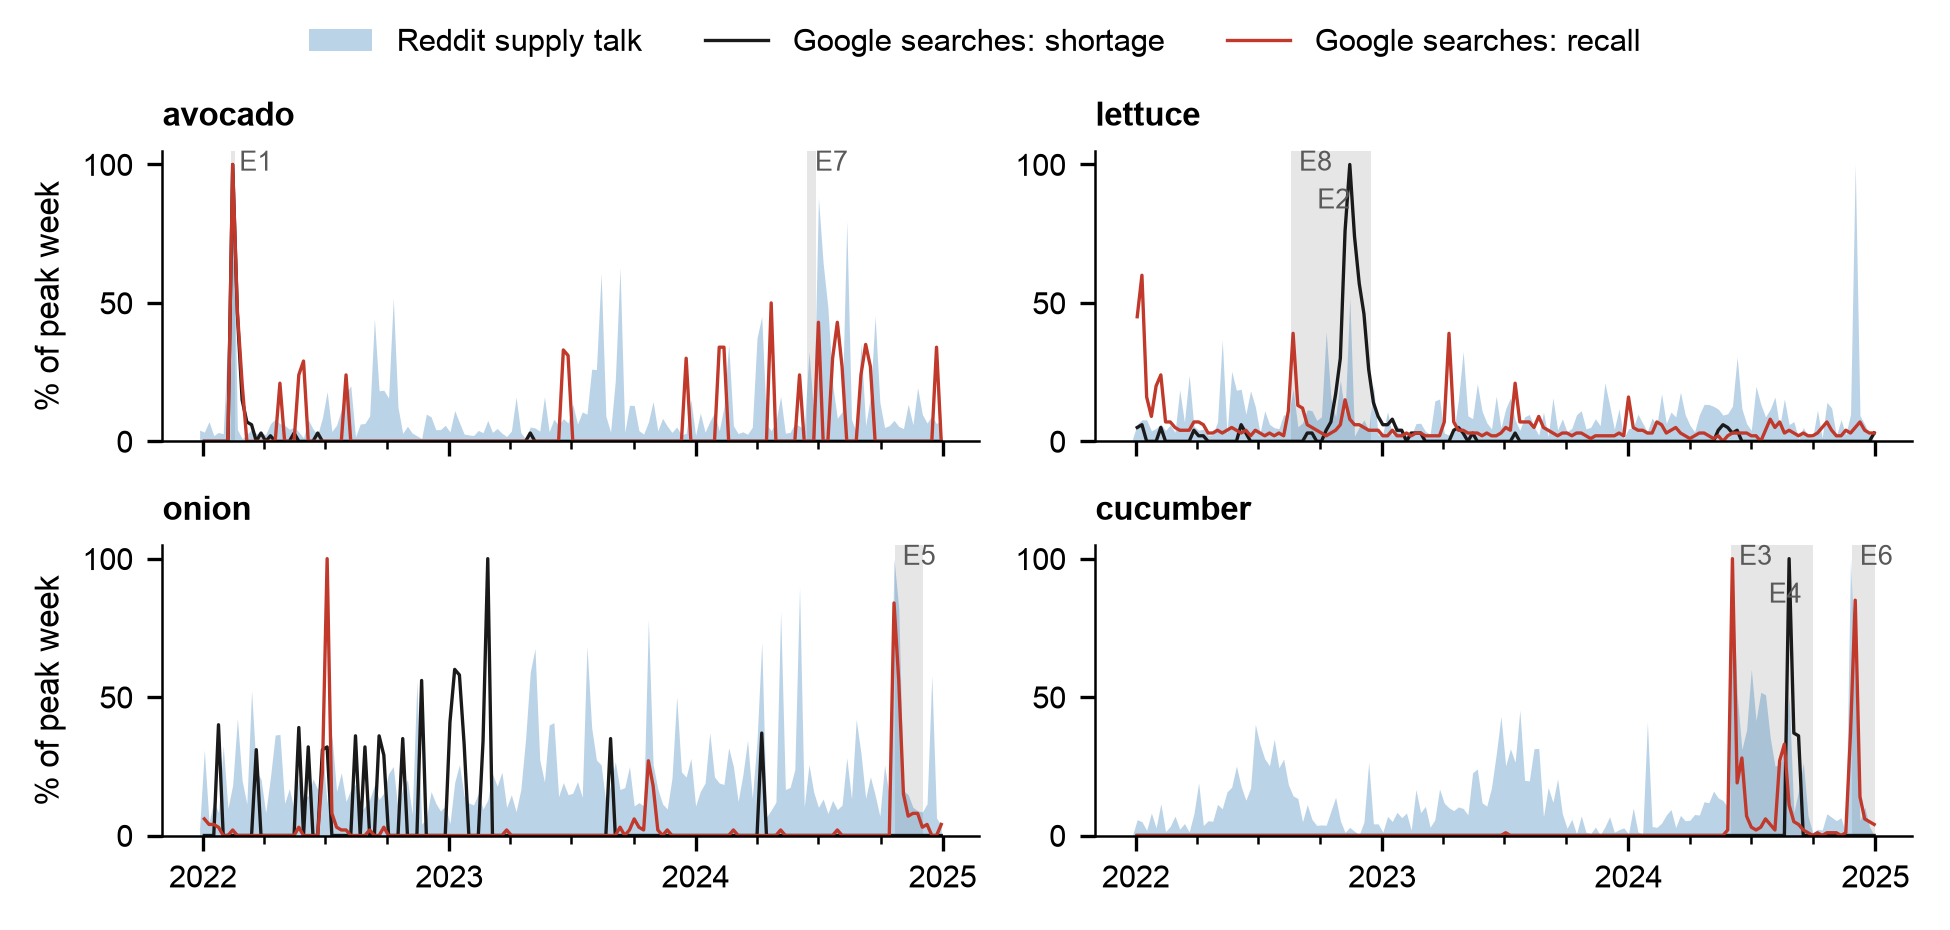
\includegraphics[width=1\linewidth,height=\textheight,keepaspectratio,alt={Reddit
supply talk and US Google searches for each product\textquotesingle s
shortage and recall, each as a share of its busiest week. Grey bands
mark the documented events.}]{../outputs/figures/google_trends.png}
\caption{Reddit supply talk and US Google searches for each
product\textquotesingle s shortage and recall, each as a share of its
busiest week within each collection period. Grey bands mark the
documented events.}
\end{figure}

\textbf{Lead and lag.} For each product and series, the weekly z-score
of the signal is correlated with that of the price index shifted by up
to eight weeks either way. Because the series are autocorrelated and the
best of 17 lags is chosen, the best correlation is tested by rotating the
signal against the price by every offset of at least 13 weeks. All
correlations are weak (\textbar r\textbar{} ≤ 0.22). Five of the 20
product--series pairs have p \textless{} 0.05, three of them in the same
week and two at a lag of seven weeks.

\subsection{F. Deliverables}\label{f.-deliverables}

\begin{table}[H]
\centering\small
\caption{Challenge deliverables in the repository.}
\begin{tabularx}{\linewidth}{l>{\RaggedRight\arraybackslash}X}
\toprule
Deliverable & File \\
\midrule
Event dataset & data/processed/event\_dataset.csv (2022--2024); event\_dataset.csv.gz in data/processed\_2019\_2021/ and data/processed\_2025\_2026/ \\
Product and event keyword list & data/processed/keyword\_dictionary.csv \\
Summary table & summary\_table.csv in each of the three data/processed* folders \\
Dataset generation code & data\_collection/ \\
Task 2 notebook & notebooks/task2\_signals\_and\_prices.ipynb \\
Environment & requirements.txt \\
Data dictionary and provenance & docs/data\_dictionary.md \\
Labels and codebook & labeling/labels.csv, labeling/codebook.md \\
\bottomrule
\end{tabularx}
\end{table}

\subsection{G. Weighting texts by upvotes or comments}\label{g.-weighting}

Each text's supply probability is multiplied by a weight from its upvotes or, for posts, its number of comments, and
the spike test of Table 4 is rerun on the weighted supply series. To pick a weighting without testing it on the same
data, it is chosen on 2019--2022 and tested on 2023--2026. The Google column does not use the list of events: it
counts Reddit supply spikes with a Google shortage or recall spike within one week. No weighting finds more events
than equal weights. The one chosen on 2019--2022, both: 1 + log(1 + upvotes + comments), finds 10 of
26 spikes near an event in 2023--2026, against 11 of 29 with
equal weights. Notebook section 13; \texttt{weighting\_robustness.csv}.

\begin{table}[htbp]
\centering\small
\caption{Reddit supply spikes under different weights. Near an event: within two weeks of a documented event. Columns 2019--22 and 2023--26: spikes near an event out of all spikes in that period. With Google: spikes with a Google shortage or recall spike within one week.}
\begin{tabular}{lccccc}
\toprule
Weight per text & Spikes & Near an event (p) & 2019--22 & 2023--26 & With Google \\
\midrule
Equal (main results) & 55 & 23 (42\%, \textless{} 0.001) & 12/26 & 11/29 & 16 (29\%) \\
\addlinespace
Upvotes: 1 + log(1 + upvotes) & 39 & 16 (41\%, 0.003) & 7/16 & 9/23 & 13 (33\%) \\
Upvotes: $\times$2 if $\geq$10 & 50 & 20 (40\%, 0.002) & 9/22 & 11/28 & 16 (32\%) \\
Upvotes: $\times$3 if $\geq$10 & 49 & 18 (37\%, 0.008) & 7/23 & 11/26 & 14 (29\%) \\
Upvotes: raw count & 50 & 18 (36\%, 0.010) & 10/28 & 8/22 & 17 (34\%) \\
\addlinespace
Comments: 1 + log(1 + comments) & 41 & 16 (39\%, 0.006) & 7/17 & 9/24 & 16 (39\%) \\
Comments: $\times$2 if $\geq$10 & 52 & 20 (38\%, 0.003) & 9/23 & 11/29 & 16 (31\%) \\
Comments: $\times$3 if $\geq$10 & 51 & 19 (37\%, 0.005) & 8/24 & 11/27 & 18 (35\%) \\
\addlinespace
Both: 1 + log(1 + upvotes + comments) & 42 & 18 (43\%, 0.001) & 8/16 & 10/26 & 14 (33\%) \\
\bottomrule
\end{tabular}
\end{table}

\subsection{H. Forecasting prices, 2019--2026}\label{h.-forecasting}

The forecasting test uses the data of Table 2 and adds daily US news
volume and tone from GDELT, FDA food recalls from openFDA and Wikipedia
pageviews.

The targets are the change in the national log price index one and four
weeks ahead, and whether the four-week change is a big move (at least
the product's 85th percentile in the training weeks). The test runs
from January 2021 to September 2026 in four-week blocks; each block uses
models trained only on weeks whose outcome was already known. Every
feature set contains price history: recent weekly changes, distance from
the 8-, 26- and 52-week means, change over a year, season and product.
The other sets add one source as z-scores against the previous eight
weeks. Ridge regression, gradient boosting and random forest were
compared for changes, and logistic regression and gradient boosting for
big moves. A block bootstrap over test weeks gives the p-values and
intervals. Code and data: \texttt{forecast\_check/}; tables
\texttt{forecast\_long\_*.csv}.

\begin{table}[htbp]
\centering\small
\caption{Forecasting the national wholesale price index, January 2021 to September 2026 (about 1,190 product-weeks). $R^2$ against a forecast of no change; AUC for big moves four weeks ahead. Each column uses the model that did best with price history alone: ridge regression (1 week), gradient boosting (4 weeks), logistic regression (AUC). With every model, no set is significantly better than price history alone (all p $\geq$ 0.07); no AUC gain exceeds 0.014, and every 95\% interval includes zero.}
\begin{tabular}{lccc}
\toprule
Features & $R^2$, 1 week & $R^2$, 4 weeks & AUC, big move \\
\midrule
\textbf{Price history only} & \textbf{0.33} & \textbf{0.23} & \textbf{0.62} \\
\addlinespace
+ Shipments & 0.33 & 0.18 & 0.61 \\
+ Reddit & 0.31 & 0.20 & 0.62 \\
+ Google Trends & 0.33 & 0.17 & 0.61 \\
+ News (GDELT) & 0.32 & 0.22 & 0.61 \\
+ FDA recalls & 0.33 & 0.22 & 0.61 \\
+ Wikipedia & 0.33 & 0.22 & 0.61 \\
+ All online sources & 0.29 & 0.17 & 0.59 \\
\bottomrule
\end{tabular}
\end{table}

\end{document}
